\section{Root Locus Design}\label{rLocus}
The Root Locus of a transfer function is a plot of all the possible positions of the closed loop poles when applying a proportional gain K. The number of poles will be the same as the ones in the open loop case and each of them will have an associated branch that shows how it moves along with K. The plot has the following main characteristics:
%
\begin{itemize}
	\item[-] The plot is symmetric with respect to the real axis.
	\item[-] The number of branches, defined as n, is equal to the number of poles in the open loop function.
	\item[-] There are m branches that end in the zeros of the open loop function, m being the number of zeros.
	\item[-] There are n-m branches going to infinity.
	\item[-] The position of the poles changes the behavior of the system as seen in \figref{rLocusStability}
\end{itemize}
%
\begin{figure}[H] 
	\centering 
	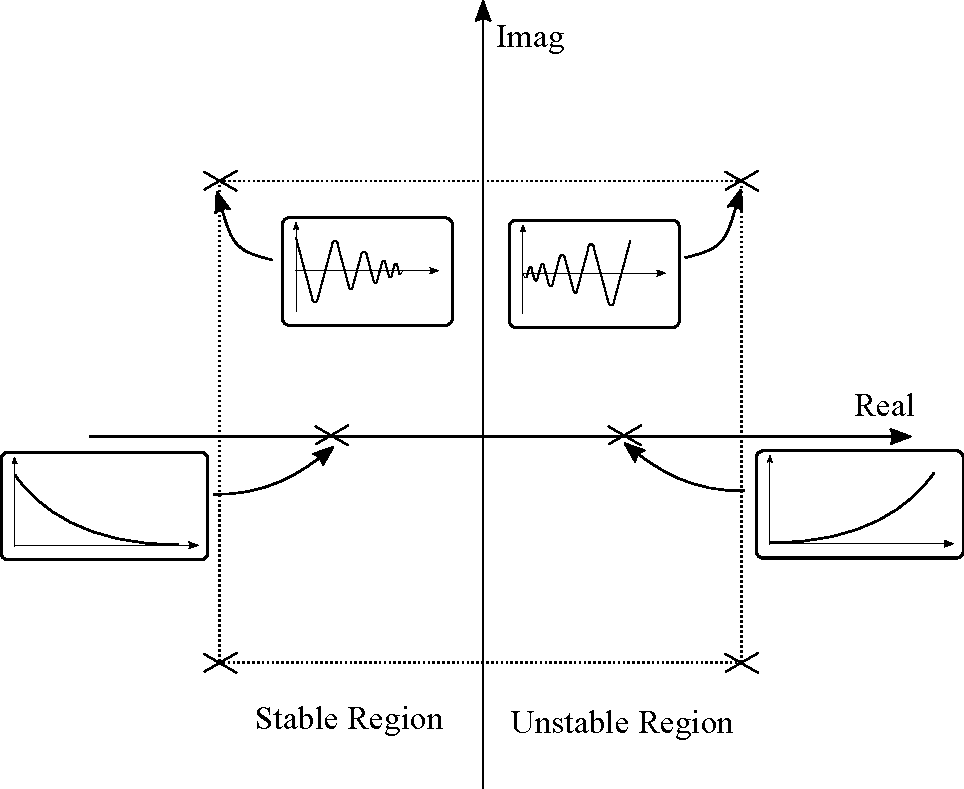
\includegraphics[scale=0.55]{figures/rLocusStability}	
	\caption{Response of a system depending on the position of its poles}
	\label{rLocusStability}
\end{figure}
%
Root Locus design of controllers is based on the fact that the closed loop poles of a system will depend on the poles, zeros and gain of the open loop function. Knowing how the plot changes with the addition of poles and zeros, the branches can be modified to place the poles of the closed loop function where needed.
